\section{Systems and Latency Design}
\label{sec:system-design}

This project is as much a systems exercise as a retrieval one. The central engineering goal is to keep the fixed-feature validation path short by moving deterministic work offline, reusing per-video artifacts across queries, and reserving expensive multimodal reasoning for a much smaller candidate set. In the repository, this design appears in both the lightweight subtitle baselines and the heavier \xml pipeline.

\Cref{fig:pipeline-overview} summarizes the staged design used in the final system. The visual structure takes inspiration from the late-fusion \xml view in the original TVR paper \cite{lei2020tvr}, but the content here is specific to the measured repository pipeline: offline subtitle-window preparation, dense text retrieval, top-$k$ video routing, and \xml refinement over aligned video and subtitle features.

\begin{figure*}[t]
  \centering
  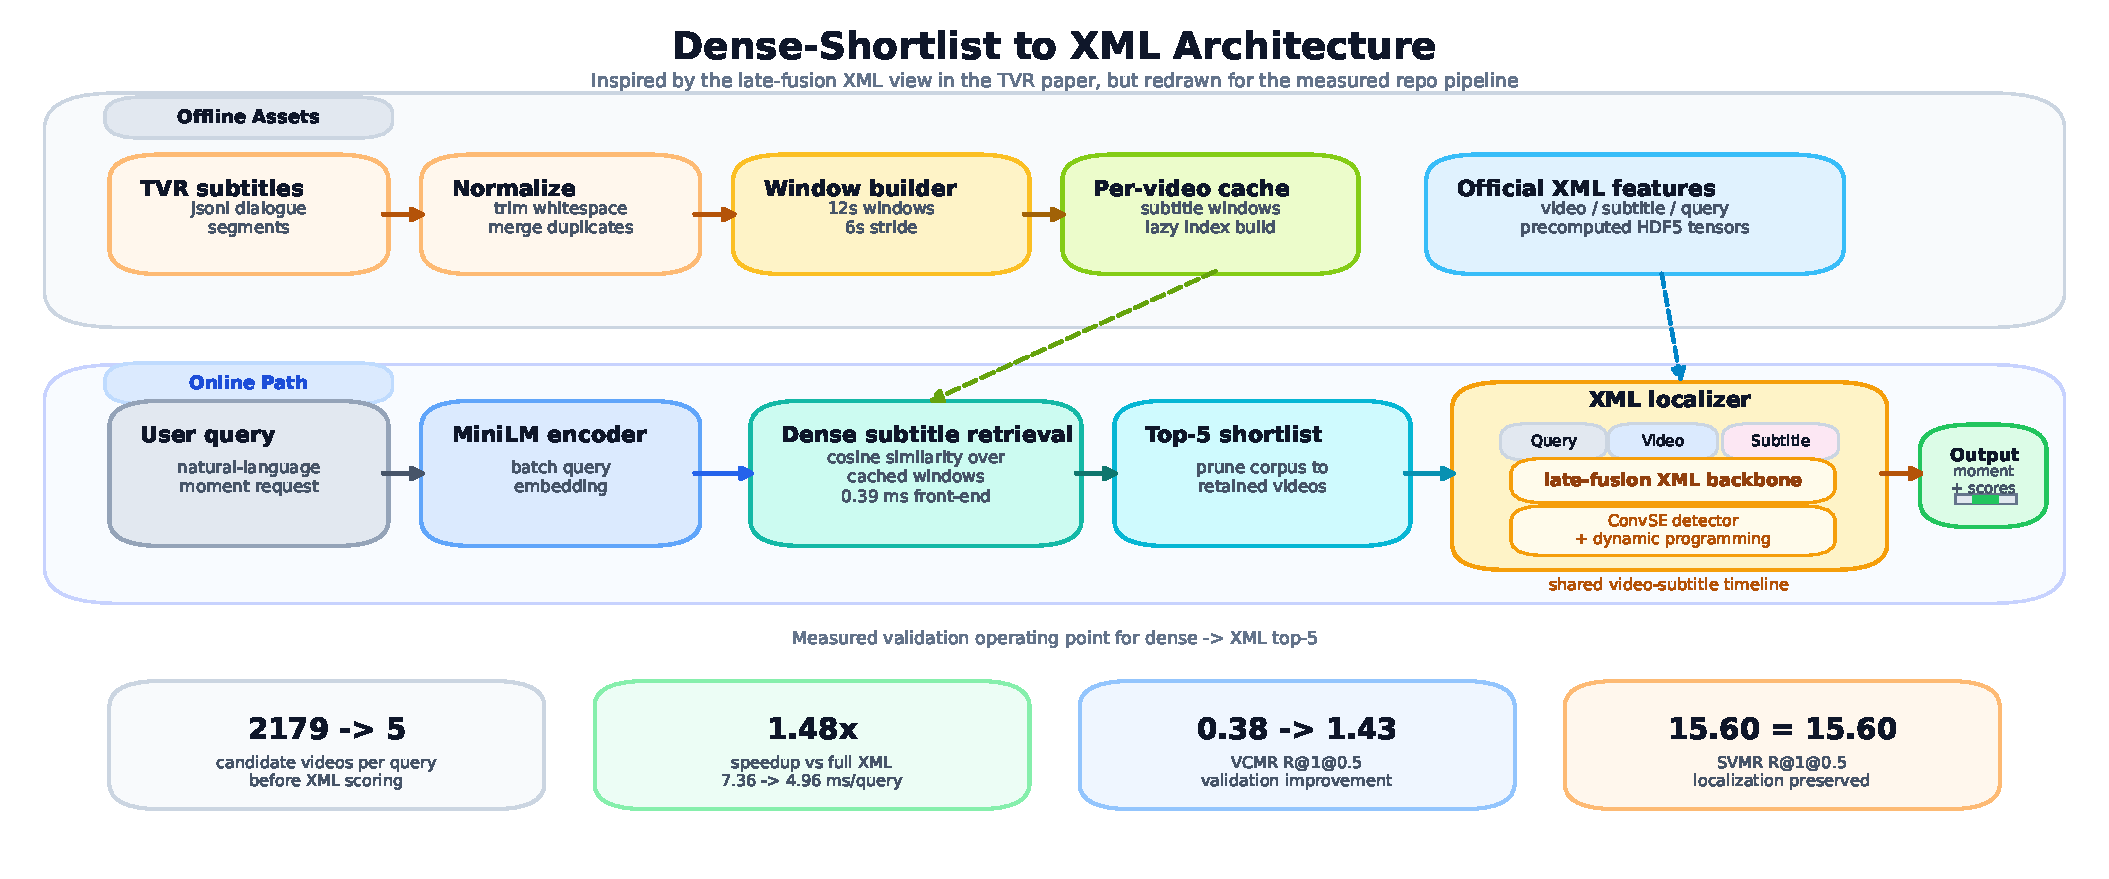
\includegraphics[width=\textwidth]{figures/pipeline_overview.pdf}
  \Description{A full-width architecture diagram of the dense video-shortlist-to-XML pipeline. The top lane shows offline subtitle normalization, window building, per-video caching, and official XML feature files. The middle lane shows the online path from a user query to MiniLM encoding, dense subtitle retrieval, a top-5 retained-video shortlist, XML localization over query, video, and subtitle streams, and the final moment output. The bottom row reports candidate pruning, speedup, VCMR improvement, and preserved SVMR accuracy for the measured validation operating point.}
  \caption{Architecture of the dense video-shortlist-to-\xml pipeline used in the final report. Dense retrieval shortlists candidate videos before official \xml scoring; shared compaction is a separate ablation, not the main method. The diagram annotates the measured fixed-feature validation operating point for dense $\rightarrow$ \xml top-5.}
  \label{fig:pipeline-overview}
\end{figure*}

\subsection{Offline Data Preparation}
The offline path begins with subtitle normalization. The window-building preprocessing script first converts the official TVR subtitle JSONL into per-video segment files. During this pass, empty rows are removed, whitespace is normalized, and consecutive duplicate subtitle strings are merged by extending their end timestamps. This step reduces redundant transcript content before retrieval is attempted.

The normalized subtitle segments are then converted into overlapping retrieval windows. In the current configuration, each window spans $12$ seconds with a stride of $6$ seconds. A window stores the video identifier, its temporal bounds, and the concatenated text from all subtitle segments that overlap that interval. Because this construction is deterministic and query-independent, it is treated entirely as preprocessing rather than query-time work.

The repository also contains a visual reranking branch, but it is not included in the final validation tables because the \clip frame-feature cache needed to reproduce that branch locally was not part of the final full-validation evaluation. For \xml, the system reuses the official precomputed video, subtitle, and query features distributed with TVR rather than extracting raw features inside this project.

One practical detail of the implementation is that the repository does not serialize separate \bm or dense subtitle indexes to disk. Instead, each evaluation script loads the prebuilt window files and lazily constructs a per-video \bm structure or dense embedding matrix the first time that video is queried. Those objects are then cached in memory and reused for subsequent queries, which avoids repeated setup cost without complicating the preprocessing pipeline.

\subsection{Online Inference Path}
For the subtitle-window baselines, the online input is a natural-language query together with a known TVR clip. The system first looks up the subtitle windows for that clip. In the \bm baseline, query-time work is limited to scoring those cached windows lexically and returning the top-$k$ spans. In the dense baseline, the query texts are encoded in batches once, the window embedding matrix is reused from cache, and retrieval reduces to a matrix-vector similarity computation followed by ranking.

The fusion branch follows the same access pattern but decomposes latency more explicitly. The code measures \bm scoring time, dense scoring time, and fusion time separately, then combines the two score streams with weighted fusion, reciprocal-rank fusion, or dense reranking over a \bm shortlist. This makes the subtitle baselines useful not only as accuracy references but also as profiling tools for understanding where query-time cost is actually spent.

The visual reranking path is kept as an exploratory branch rather than part of the final evaluated method. It rescored dense subtitle candidates with precomputed \clip frame embeddings, but the final validation tables focus on dense video routing before \xml.

The main \xml path uses the official inference code over the provided HDF5 features, with dense retrieval passed in as an external video-ranking file. The \xml evaluator then limits VCMR scoring to the configured top-$k$ videos for each query. This is the measured dense-shortlist-to-\xml pipeline: it changes which candidate videos reach \xml, but it does not redesign the \xml localization architecture.

The shared-compaction path is a separate ablation. There, the repository slices the video and subtitle streams on the same retained timeline before context encoding. The selected indices are stored as \texttt{retained\_clip\_indices}, both modalities are sliced with those indices, and inference later maps predicted compact start/end positions back to timestamps on the original clip grid. A contiguity mask ensures that predicted spans cannot cross gaps introduced by compaction. This tests whether temporal compression inside \xml helps as an alternative or add-on to routing, and the results show that the current selector is too crude.

\subsection{Validation Runtime Reduction Strategies}
Several concrete design choices in the repository target fixed-feature validation runtime directly.

\paragraph{Shift immutable work offline.}
Subtitle parsing and window construction are query-independent, so they are removed from the critical path. This is especially important in TVR because transcript cleanup would otherwise dominate a fair fixed-feature retrieval-runtime measurement.

\paragraph{Cache aggressively at the video level.}
The baselines are evaluated over many queries that revisit the same clips. The implementation therefore caches BM25 state, dense subtitle embeddings, and visual features per video after first use. Dense query embeddings are also batched ahead of the main retrieval loop, so the per-query online cost is closer to lookup and scoring than to full re-encoding of every artifact.

\paragraph{Apply expensive models only to shortlists.}
The final system applies the same principle at video scale: dense retrieval chooses a small top-$k$ set, and \xml spends its cross-modal budget there. Shared compaction tests the harder temporal version of this idea, but the stronger measured result comes from video-level routing.

\paragraph{Keep runtime fixes separate from modeling claims.}
The \xml wrappers also include environment-level adjustments needed to make official validation practical on the available machine, such as resolving local feature paths and running with \texttt{--no\_core\_driver} to avoid copying large HDF5 feature files into RAM. These choices matter for reproducibility and validation wall-clock time, but they do not change the underlying \xml model.

\begin{table}[t]
  \centering
  \caption{Average online latency for the reported dense-shortlist-to-XML top-5 validation pipeline. Offline document encoding, subtitle parsing, window construction, and feature extraction are excluded. XML localization is estimated as the residual between end-to-end wall time and the measured retrieval front-end.}
  \label{tab:latency-breakdown}
  \begin{tabular}{p{0.24\linewidth}p{0.44\linewidth}c}
    \toprule
    Stage & Description & Time (ms) \\
    \midrule
    Query encoding & MiniLM text encoding averaged over the validation sweep & 0.22 \\
    Candidate generation & No separate lexical prefilter in the dense-top5 pipeline & 0.00 \\
    Dense shortlist scoring & Subtitle-embedding similarity and top-5 ranking & 0.17 \\
    Visual reranking & Disabled in the reported pipeline & 0.00 \\
    XML localization & Cross-modal localization on the top-5 shortlist (residual estimate) & 4.57 \\
    \midrule
    Total & End-to-end wall time per query for dense shortlist $\rightarrow$ XML & 4.96 \\
    \bottomrule
  \end{tabular}
\end{table}

